\section{Expedition Logistics}


    \begin{marginfigure}
\checkoddpage \ifoddpage \forcerectofloat \else \forceversofloat \fi
\centering
 \frame{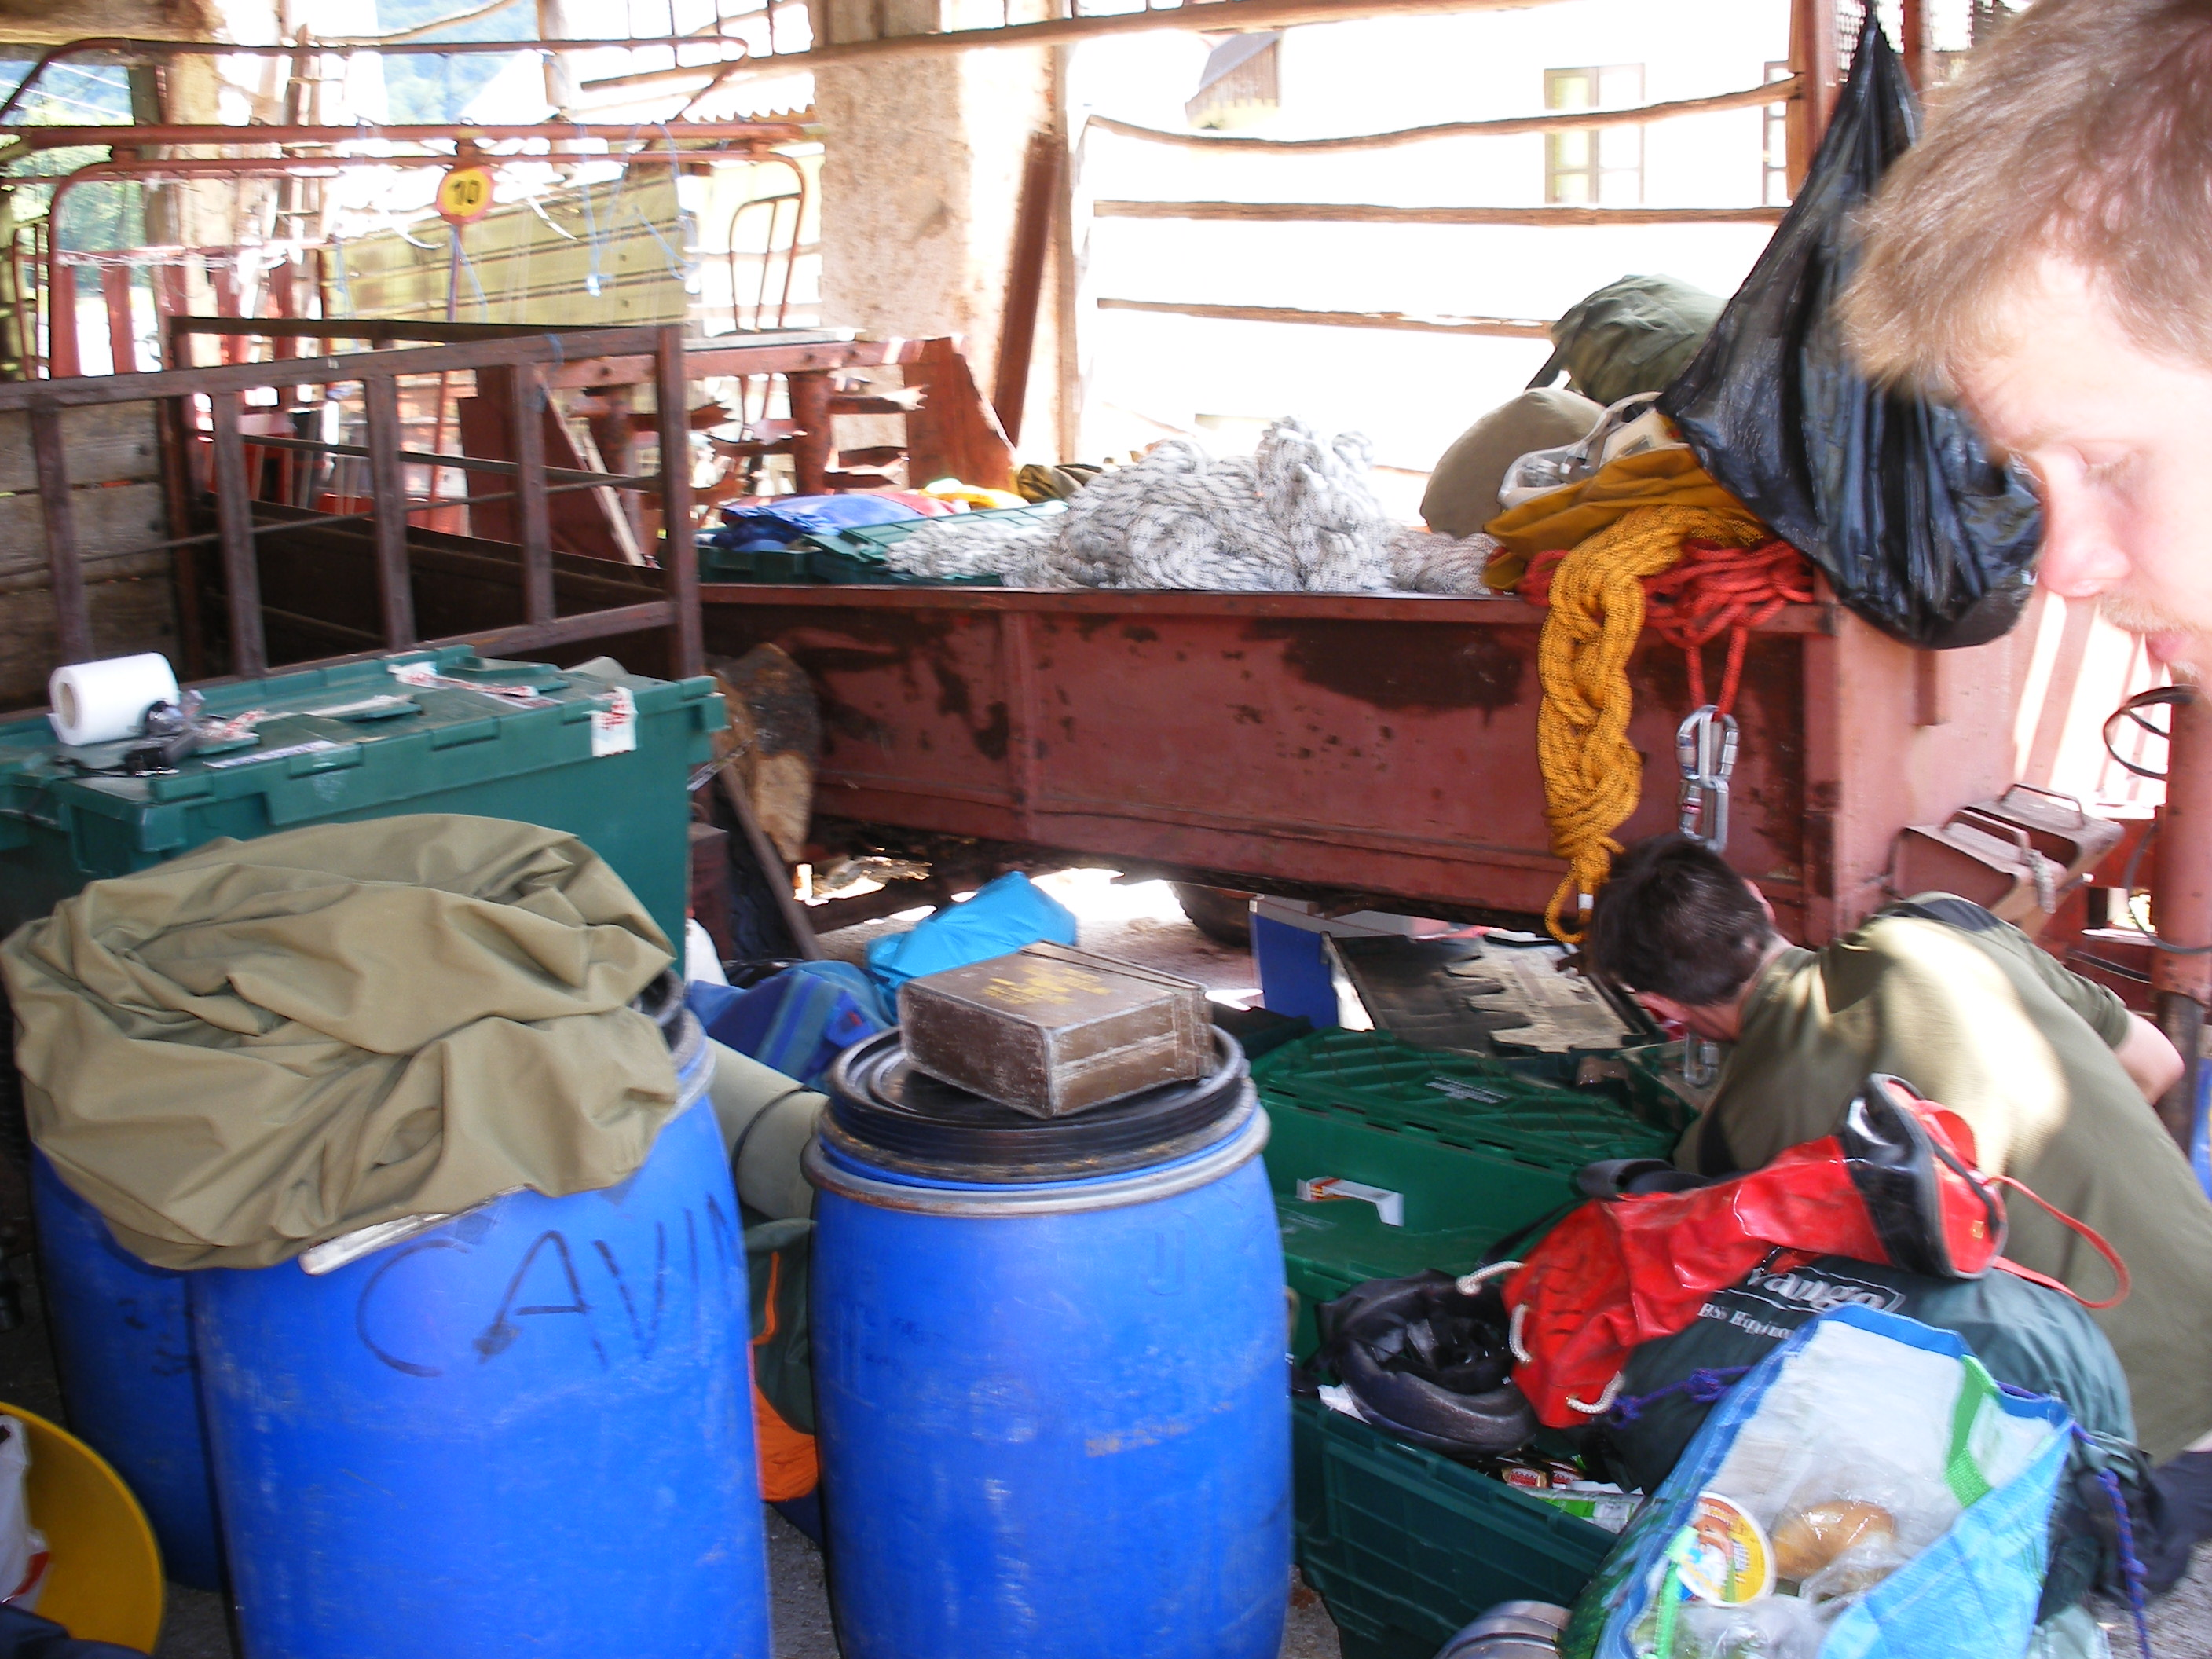
\includegraphics[width=\linewidth]{2010/expo_logistics/Mike Foley 05--orig.jpg}} 
 \caption{The Skalar family's barn becomes organised chaos when the expedition takes over for a few weeks. \pic{Mike Foley}}
 \label{Skalar barn}
\end{marginfigure}

A nine seater minibus was hired from Imperial College Union for four weeks and two days. 
This was driven
non-stop from \passage[town]{South Kensington} to \passage[town]{Tolmin}, Slovenia in just under 24 hours
including the ferry journey (Friday -- Saturday evening). Special permission
had been acquired by the JSPDT to camp in the national park, on top of \passage[mountain]{Tolminski Migovec}
in our usual bivouac spot. The van made two trips to \passage[town]{Tolminske Ravne} (912 m) on
Sunday morning, where the equipment was unloaded into the barn of the Skalar
family. 

The mountaintop was in continual occupation from Sunday evening, with the first
caving trips on Tuesday.

\subsection{Caving Logistics}

The main route to \passage{Friendship Gallery} in \passage{Vrtnarija} contains over 500
m of vertical pitches. Many of these ropes had been in place for some time and it was decided to replace them. Six hundred metres of new ropes were installed in the first few days of caving thanks to concerted effort, multiple waves of rigging teams and an 'all hands on deck' attitude
from the whole expedition team.  Other factors that aided a quick start to the
exploration were:


\tweet{4:55PM Jul 13, 2010}{T-3 days.Adv party fly out 2day (JKP,WF,JH) to get H20.We're expecting 68 caver-weeks in total.Weather pushing mid 30s with thunder storms.}

\begin{itemize}
\item the significant amounts of dried foods left in loco at the bivouac
site on \passage[mountain]{Migovec} (thereby saving on porterage time at the beginning of expedition); 
\item the sending of an 'advance party' to set up the bivouac and collect drinking water (a day of back breaking snow haulage) before the main group arrived; 
\item the fact that all underground camping kit was carefully packed in transport sacks in England. 
\end{itemize}
These logistical steps meant that within the first week of the main expedition group arriving in Slovenia most of the porterage had been done, the cave had been re-rigged and a 4-bed underground camp at the \passage{X-Ray} (-550m) site had been set up. In fact, the very first survey
data was recorded at -606m exactly seven and a half days after the van left \passage[town]{South Kensington}.


\subsection{Expedition Talks}

    \begin{marginfigure}
\checkoddpage \ifoddpage \forcerectofloat \else \forceversofloat \fi
\centering
 \frame{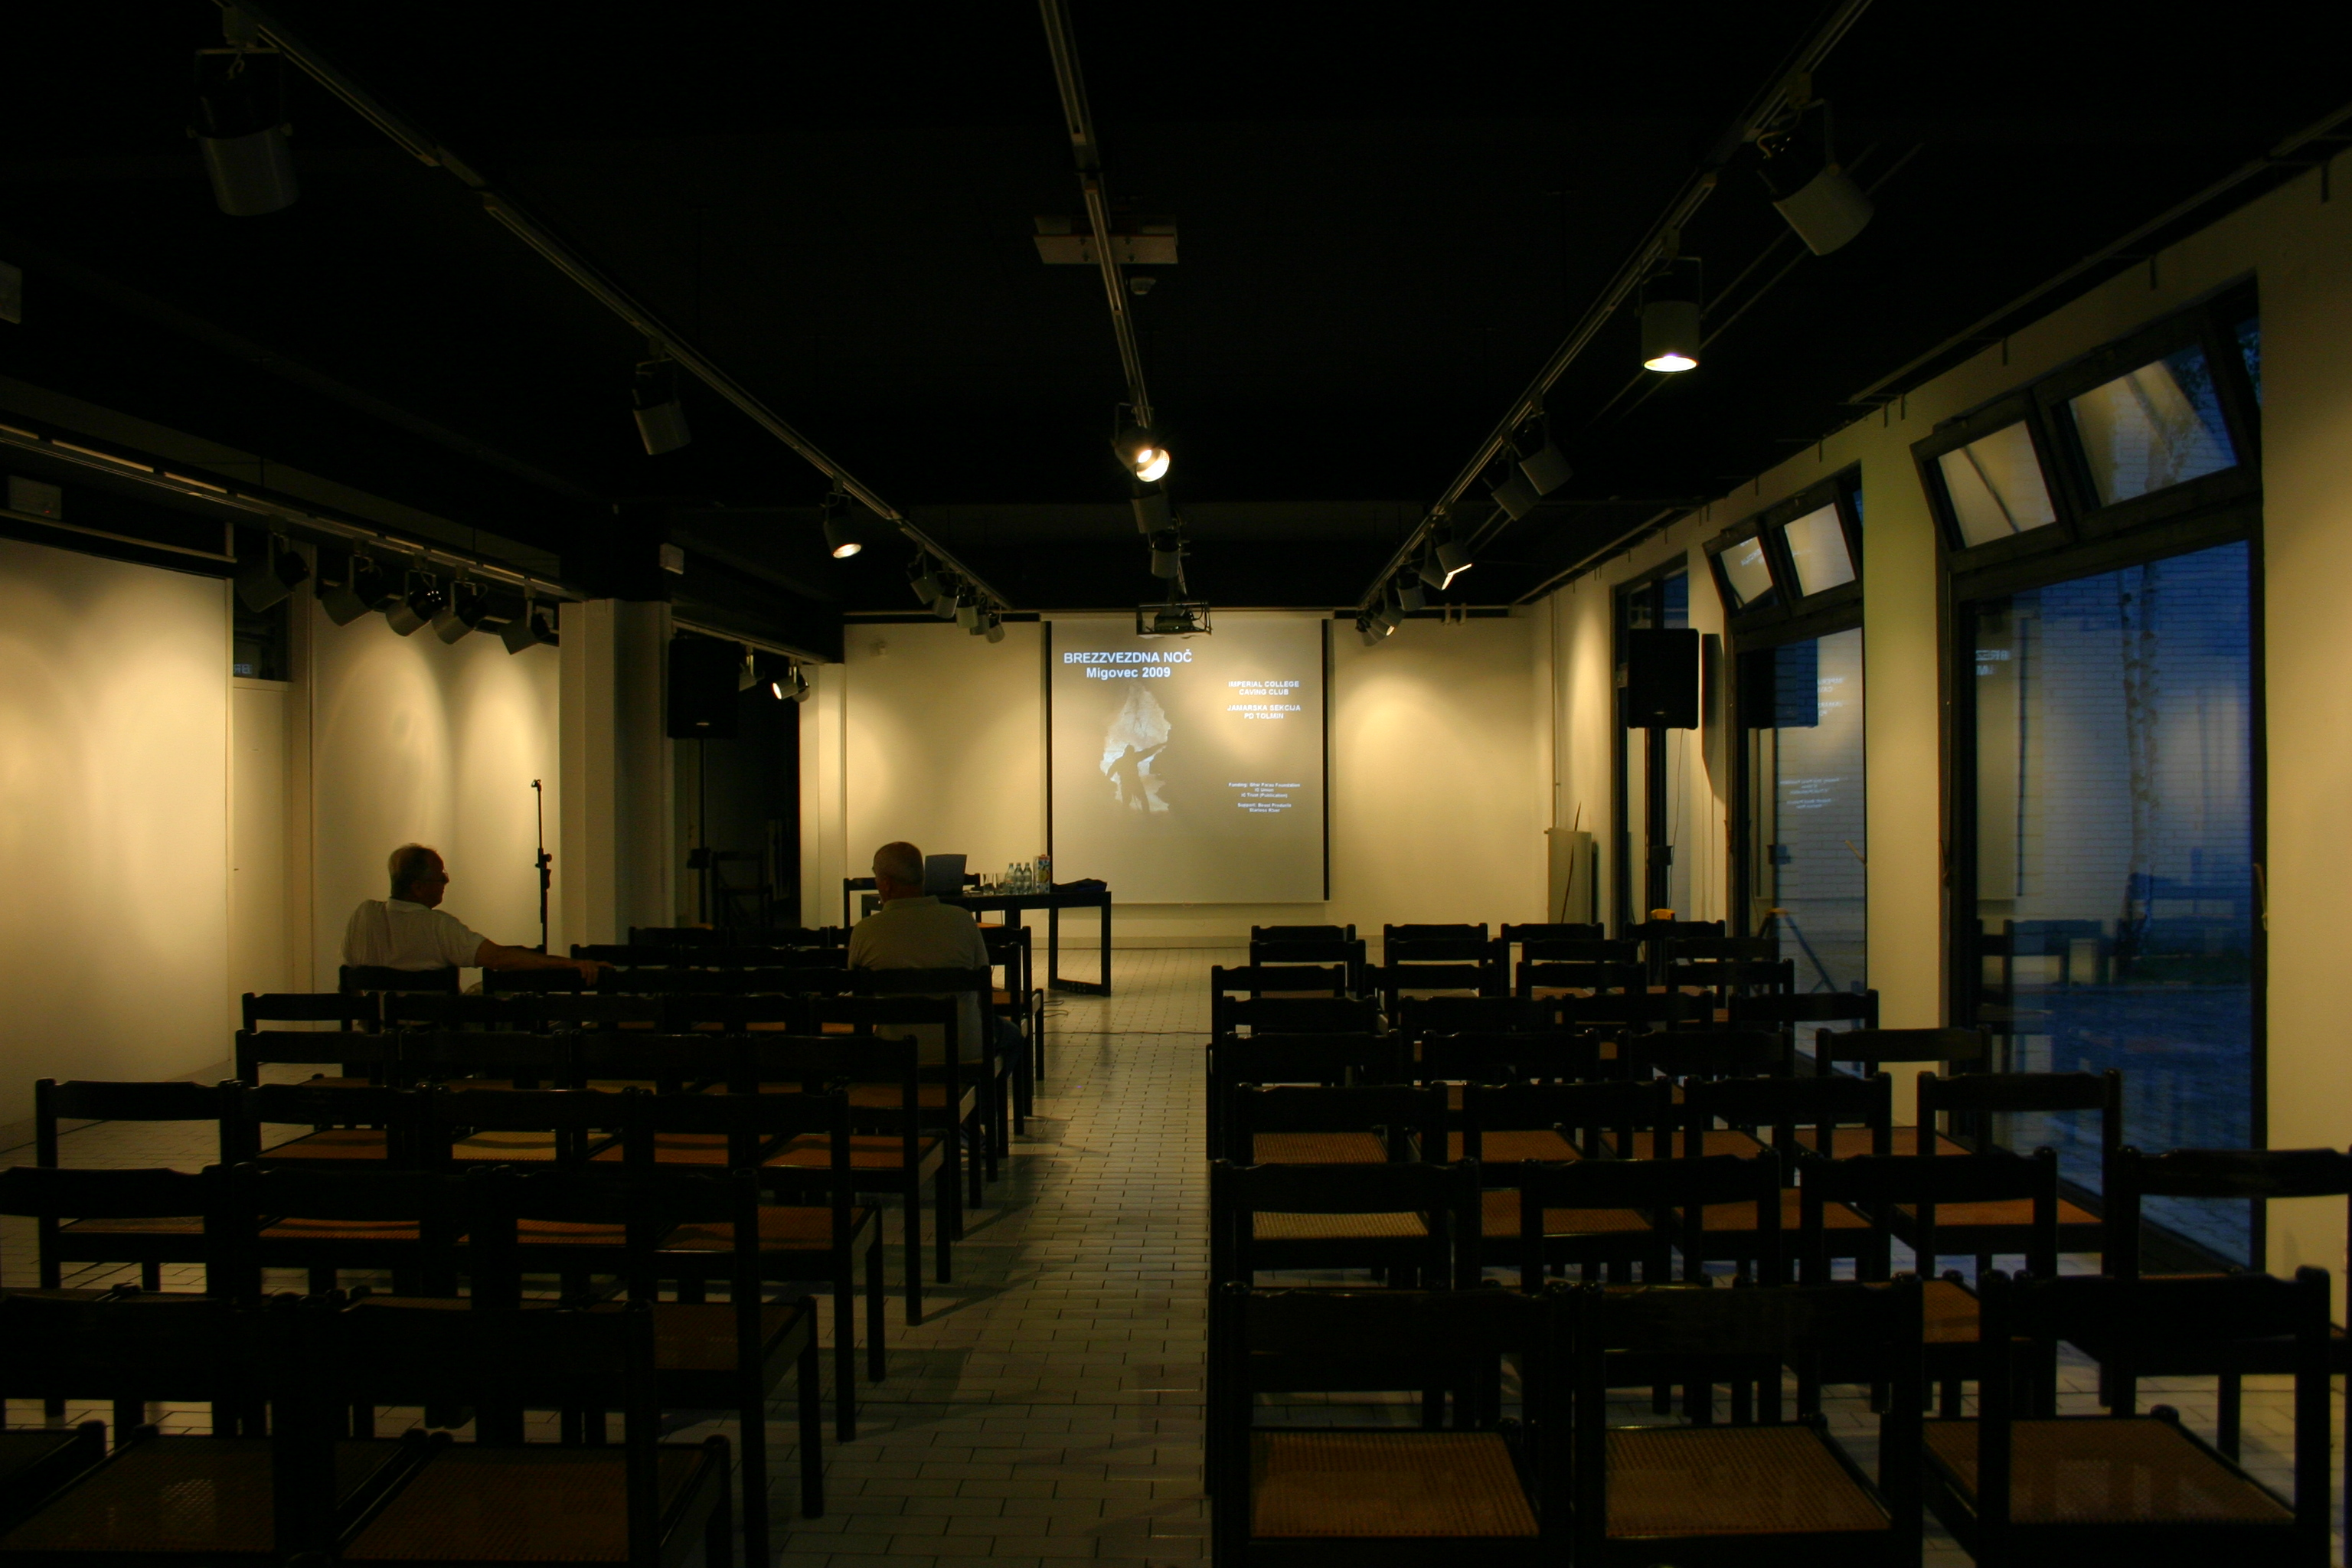
\includegraphics[width=\linewidth]{2010/expo_logistics/2009-08-23-01.09.43 - Tharatorn Supasiti - Slideshow setup--orig.jpg}} 
 \caption{It was typical of this era for the \passage{Migovec} cavers to present a slideshow regarding the year's discoveries in the \protect\passage[town]{Tolmin} library at the end of expedition. \pic{Tharatorn Supasiti}}
 \label{Tolmin slideshow 2009}
\end{marginfigure}

An expedition slideshow was given by Jarvist Frost, with translation by Jana Čarga, on the Saturday evening at the end of expedition before departing.

An expedition talk was presented by Jarvist Frost at Hidden Earth 2010.




\section{Rope Testing}

The rope removed from the main pitch series in \passage{Vrtnarija} is currently being
drop tested by Bob Mehew on the British Caving Association rope testing rig. This will hopefully provide some useful information the extent of degradation of SRT ropes used in
Alpine exploration, and the associated `permanent' rigging.
